
\gaokaoheader{2020}{山东卷}


\gaokaoxz

%一、单项选择题:本题共 $ 8 $ 小题,每小题 $ 3 $ 分,共 $ 24 $ 分。每小题只有一个选项符合题目要求。

\begin{enumerate}
%\renewcommand{\labelenumi}{\arabic{enumi}.}
% A(\Alph) a(\alph) I(\Roman) i(\roman) 1(\arabic)
%设定全局标号series=example	%引用全局变量resume=example
%[topsep=-0.3em,parsep=-0.3em,itemsep=-0.3em,partopsep=-0.3em]
%可使用leftmargin调整列表环境左边的空白长度 [leftmargin=0em]
\item
一质量为 $ m $ 的乘客乘坐竖直电梯下楼,其位移 $ s $ 与时间 $ t $ 的关系图像如图所示。乘客所受支持力的大小
用 $ F_{N} $ 表示,速度大小用 $ v $ 表示。重力加速度大小为 $ g $。以下判断正确的是 \xzanswer{D} 
\begin{figure}[h!]
\centering
\includesvg[width=0.23\linewidth]{picture/svg/GZ-3-tiyou-0729}
\end{figure}


\fourchoices
{$ 0 \sim t_{1} $ 时间内,$ v $ 增大,$ F_{N} >mg $}
{$ t_{1} \sim t_{2} $ 时间内,$ v $ 减小,$ F_{N} <mg $}
{$ t_{2} \sim t_{3} $ 时间内,$ v $ 增大,$ F_{N} <mg $}
{$ t_{2} \sim t_{3} $ 时间内,$ v $ 减小,$ F_{N} >mg $}


%题目类型:选择
%题目难度:8.5
%题目区域:运动定律:超重失重
%思想方法:
%题目特征:图像分析
%题目备注:



\item
氚核 \ce{^{3}_{1}H} 发生$ \beta $衰变成为氦核 \ce{^{3}_{2}He} 。假设含氚材料中 \ce{^{3}_{2}He} 发生$ \beta $衰变产生的电子可以全部定向移动,在 $ 3.2 \times 10^{4} \ s $ 时间内形成的平均电流为 $ 5.0 \times 10^{-8} \ A $。已知电子电荷量为 $ 1.6 \times 10^{-19} \ C $,在这段时间内发生$ \beta $衰变的
氚核 \ce{^{3}_{1}H} 的个数为 \xzanswer{B} 

\fourchoices
{$5.0 \times 10^{14}$}
{$1.0 \times 10^{16}$}
{$ 2.0 \times 10^{16}$}
{$1.0 \times 10^{18}$}


%题目类型:选择
%题目难度:8
%题目区域:原子物理
%思想方法:
%题目特征:材料分析
%题目备注:




\item
双缝干涉实验装置的截面图如图所示。光源 $ S $ 到 $ S_{1} $、$ S_{2} $ 的距离相等,$ O $ 点为 $ S_{1} $、$ S_{2} $ 连线中垂线与光屏的
交点。光源 $ S $ 发出的波长为 $ \lambda $ 的光,经 $ S_{1} $ 出射后垂直穿过玻璃片传播到 $ O $ 点,经 $ S_{2} $ 出射后直接传播到
$ O $ 点,由 $ S_{1} $ 到 $ O $ 点与由 $ S_{2} $ 到 $ O $ 点,光传播的时间差为 $ \Delta t $。玻璃片厚度为 $ 10\lambda $,玻璃对该波长光的折射
率为 $ 1.5 $,空气中光速为 $ c $,不计光在玻璃片内的反射。以下判断正确的是 \xzanswer{A} 
\begin{figure}[h!]
\centering
\includesvg[width=0.3\linewidth]{picture/svg/GZ-3-tiyou-0730}
\end{figure}


\fourchoices
{$\Delta t=\frac{5 \lambda}{c}$}
{$ \Delta t=\frac{15 \lambda}{2 c}$}
{$ \Delta t=\frac{10 \lambda}{c}$}
{$ \Delta t=\frac{15 \lambda}{c}$}

%题目类型:选择
%题目难度:7.5
%题目区域:光学:光的干涉
%思想方法:
%题目特征:
%题目备注:




\item
一列简谐横波在均匀介质中沿 $ x $ 轴负方向传播,
已知 $ x= \frac{ 5 }{ 4 } \lambda $ 处质点的振动方程为 $y=A \cos \left(\frac{2 \pi}{T} t\right)$,
则$ t= \frac{ 3 }{ 4 } T $
时刻的波形图正确的是 \xzanswer{D} 

\pfourchoices
{\includesvg[width=3.3cm]{picture/svg/GZ-3-tiyou-0731}}
{\includesvg[width=3.3cm]{picture/svg/GZ-3-tiyou-0732}}
{\includesvg[width=3.3cm]{picture/svg/GZ-3-tiyou-0733}}
{\includesvg[width=3.3cm]{picture/svg/GZ-3-tiyou-0734}}



%题目类型:选择
%题目难度:7.5
%题目区域:机械波:波的描述
%思想方法:
%题目特征:图像选择
%题目备注:




\item
图 \subref{2020:山东:5a} 中的理想变压器原、副线圈匝数比 $ n_{1}:n_{2}=22:3 $,输入端 $ a $、$ b $ 所接电压 $ u $ 随时间 $ t $ 的变化关系如图 \subref{2020:山东:5b} 所示。灯泡 $ L $ 的电阻恒为 $ 15 \ \Omega $,额定电压为 $ 24 \ V $。定值电阻 $ R_{1} =10 \ \Omega $、$ R_{2} =5 \ \Omega $, 滑动变阻器 $ R $ 的最
大阻值为 $ 10 \ \Omega $。为使灯泡正常工作,滑动变阻器接入电路的电阻应调节为 \xzanswer{A} 

\begin{figure}[h!]
\centering
\begin{subfigure}{0.4\linewidth}
\centering
\includesvg[width=0.8\linewidth]{picture/svg/GZ-3-tiyou-0735} 
\caption{}\label{2020:山东:5a}
\end{subfigure}
\begin{subfigure}{0.4\linewidth}
\centering
\includesvg[width=0.8\linewidth]{picture/svg/GZ-3-tiyou-0736} 
\caption{}\label{2020:山东:5b}
\end{subfigure}	
\end{figure}


\fourchoices
{$ 1 \ \Omega $}
{$ 5 \ \Omega $}
{$ 6 \ \Omega $}
{$ 8 \ \Omega $}

%题目类型:选择
%题目难度:7
%题目区域:电磁感应:变压器与高压输电
%思想方法:
%题目特征:
%题目备注:




\item
一定质量的理想气体从状态 $ a $ 开始,经 $ a \rightarrow b $、$ b \rightarrow c $、$ c \rightarrow a $ 三个过程后回到初始状态 $ a $,其 $ p-V $ 图像如图
所示。已知三个状态的坐标分别为 $ a $($ V_{0} $, $ 2p_0 $)、 $ b $($ 2V_0 $,$ p_{0} $)、$ c $($ 3V_0 $, $ 2p_0 $) 以下判断正确的是 \xzanswer{C} 
\begin{figure}[h!]
\centering
\includesvg[width=0.26\linewidth]{picture/svg/GZ-3-tiyou-0737}
\end{figure}


\fourchoices
{气体在 $ a \rightarrow b $ 过程中对外界做的功小于在 $ b \rightarrow c $ 过程中对外界做的功}
{气体在 $ a \rightarrow b $ 过程中从外界吸收的热量大于在 $ b \rightarrow c $ 过程中从外界吸收的热量}
{在 $ c \rightarrow a $ 过程中,外界对气体做的功小于气体向外界放出的热量}
{气体在 $ c \rightarrow a $ 过程中内能的减少量大于 $ b \rightarrow c $ 过程中内能的增加量}


%题目类型:选择
%题目难度:5
%题目区域:热学:热力学第一定律:理想气体状态方程
%思想方法:
%题目特征:图像分析
%题目备注:



\item
我国将在今年择机执行“天问 $ 1 $ 号”火星探测任务。质量为 $ m $ 的着陆器在着陆火星前,会在火星表面附近
经历一个时长为 $ t_{0} $、速度由 $ v_{0} $ 减速到零的过程。已知火星的质量约为地球的 $ 0.1 $ 倍,半径约为地球的 $ 0.5 $倍,地球表面的重力加速度大小为 $ g $,忽略火星大气阻力。若该减速过程可视为一个竖直向下的匀减
速直线运动,此过程中着陆器受到的制动力大小约为 \xzanswer{B} 

\fourchoices
{$m\left(0.4 g-\frac{v_{0}}{t_{0}}\right)$}
{$ m\left(0.4 g+\frac{v_{0}}{t_{0}}\right)$}
{$ m\left(0.2 g-\frac{v_{0}}{t_{0}}\right)$}
{$ m\left(0.2 g+\frac{v_{0}}{t_{0}}\right)$}


%题目类型:选择
%题目难度:6.5
%题目区域:万有引力
%思想方法:
%题目特征:材料分析
%题目备注:




\item
如图所示,一轻质光滑定滑轮固定在倾斜木板上,质量分别为 $ m $ 和 $ 2m $ 的物块 $ A $、$ B $,通过不可伸长的轻
绳跨过滑轮连接,$ A $、$ B $ 间的接触面和轻绳均与木板平行。$ A $ 与 $ B $ 间、$ B $ 与木板间的动摩擦因数均为$ \mu $,
设最大静摩擦力等于滑动摩擦力。当木板与水平面的夹角为 $ 45 ^{ \circ } $时,物块 $ A $、$ B $ 刚好要滑动,则$ \mu $的值为 \xzanswer{C} 
\begin{figure}[h!]
\centering
\includesvg[width=0.27\linewidth]{picture/svg/GZ-3-tiyou-0738}
\end{figure}

\fourchoices
{$\frac{1}{3}$}
{$\frac{1}{4}$}
{$\frac{1}{5}$}
{$\frac{1}{6}$}


%题目类型:选择
%题目难度:5.5
%题目区域:相互作用
%思想方法:假设
%题目特征:计算练习
%题目备注:




%二、多项选择题:本题共 $ 4 $ 小题,每小题 $ 4 $ 分,共 $ 16 $ 分。每小题有多个选项符合题目要求。全部选对得 $ 4 $ 分,选对但不全的得 $ 2 $ 分,有选错的得 $ 0 $ 分。


\item
截面为等腰直角三角形的三棱镜如图 \subref{2020:山东:9a} 所示。$ DE $ 为嵌在三棱镜内部紧贴 $ BB ^{\prime} C ^{\prime} C $ 面的线状单色可见光光
源,$ DE $ 与三棱镜的 $ ABC $ 面垂直,$ D $ 位于线段 $ BC $ 的中点。图 \subref{2020:山东:9b} 为图 \subref{2020:山东:9a} 中 $ ABC $ 面的正视图。三棱镜对
该单色光的折射率为 $ 2 $,只考虑由 $ DE $ 直接射向侧面 $ AA ^{\prime} C ^{\prime} C $ 的光线。下列说法正确的是 \xzanswer{AC} 
\begin{figure}[h!]
\centering
\begin{subfigure}{0.3\linewidth}
\centering
\includesvg[width=0.8\linewidth]{picture/svg/GZ-3-tiyou-0739} 
\caption{}\label{2020:山东:9a}
\end{subfigure}
\begin{subfigure}{0.3\linewidth}
\centering
\includesvg[width=0.8\linewidth]{picture/svg/GZ-3-tiyou-0740} 
\caption{}\label{2020:山东:9b}
\end{subfigure}
\end{figure}


\fourchoices
{光从 $ AA ^{\prime} C ^{\prime} C $ 面出射的区域占该侧面总面积的$ \frac{ 1 }{ 2 } $}
{光从 $ AA ^{\prime} C ^{\prime} C $ 面出射的区域占该侧面总面积的$ \frac{ 2 }{ 3 } $}
{若 $ DE $ 发出的单色光频率变小,$ AA ^{\prime} C ^{\prime} C $ 面有光出射的区域面积将增大}
{若 $ DE $ 发出的单色光频率变小,$ AA ^{\prime} C ^{\prime} C $ 面有光出射的区域面积将减小}

%题目类型:选择
%题目难度:7
%题目区域:光学:光的折射
%思想方法:
%题目特征:
%题目备注:




\item
真空中有两个固定的带正电的点电荷,电荷量不相等。一个带负电的试探电荷置于二者连线上的 $ O $ 点
时,仅在电场力的作用下恰好保持静止状态。过 $ O $ 点作两正电荷连线的垂线,以 $ O $ 点为圆心的圆与连
线和垂线分别交于 $ a $、$ c $ 和 $ b $、$ d $,如图所示。以下说法正确的是 \xzanswer{BD} 
\begin{figure}[h!]
\centering
\includesvg[width=0.39\linewidth]{picture/svg/GZ-3-tiyou-0741}
\end{figure}


\fourchoices
{$ a $ 点电势低于 $ O $ 点}
{$ b $ 点电势低于 $ c $ 点}
{该试探电荷在 $ a $ 点的电势能大于在 $ b $ 点的电势能}
{该试探电荷在 $ c $ 点的电势能小于在 $ d $ 点的电势能}


%题目类型:选择
%题目难度:5
%题目区域:电场:电场强度:电势能
%思想方法:
%题目特征:
%题目备注:




\item
如图所示,质量为 $ M $ 的物块 $ A $ 放置在光滑水平桌面上,右侧连接一固定于墙面的水平轻绳,左侧通过
一倾斜轻绳跨过光滑定滑轮与一竖直轻弹簧相连。现将质量为 $ m $ 的钩码 $ B $ 挂于弹簧下端,当弹簧处于
原长时,将 $ B $ 由静止释放,当 $ B $ 下降到最低点时(未着地),$ A $ 对水平桌面的压力刚好为零。轻绳不
可伸长,弹簧始终在弹性限度内,物块 $ A $ 始终处于静止状态。以下判断正确的是 \xzanswer{ACD} 
\begin{figure}[h!]
\centering
\includesvg[width=0.28\linewidth]{picture/svg/GZ-3-tiyou-0742}
\end{figure}


\fourchoices
{$ M<2m $}
{$ 2m<M<3 \ m $}
{在 $ B $ 从释放位置运动到最低点的过程中,所受合力对 $ B $ 先做正功后做负功}
{在 $ B $ 从释放位置运动到速度最大的过程中,$ B $ 克服弹簧弹力做的功等于 $ B $ 机械能的减少量}



%题目类型:选择
%题目难度:7
%题目区域:相互作用:能量守恒:机械能守恒
%思想方法:
%题目特征:
%题目备注:



\item 
如图所示,平面直角坐标系的第一和第二象限分别存在磁感应强度大小相等、方向相反且垂直于坐标
平面的匀强磁场,图中虚线方格为等大正方形。一位于 $ Oxy $ 平面内的刚性导体框 $ abcde $ 在外力作用下
以恒定速度沿 $ y $ 轴正方向运动(不发生转动)。从图示位置开始计时,$ 4 \ s $ 末 $ bc $ 边刚好进入磁场。在
此过程中,导体框内感应电流的大小为 $ I $ , $ ab $ 边所受安培力的大小为 $ F_{ab} $,二者与时间 $ t $ 的关系图像,
可能正确的是 \xzanswer{BC} 
\begin{figure}[h!]
\centering
\includesvg[width=0.28\linewidth]{picture/svg/GZ-3-tiyou-0743}
\end{figure}

\pfourchoices
{\includesvg[width=3cm]{picture/svg/GZ-3-tiyou-0744}}
{\includesvg[width=3cm]{picture/svg/GZ-3-tiyou-0745}}
{\includesvg[width=3cm]{picture/svg/GZ-3-tiyou-0746}}
{\includesvg[width=3cm]{picture/svg/GZ-3-tiyou-0747}}

%题目类型:选择
%题目难度:5.5
%题目区域:磁场:安培力:电磁感应:电磁感应定律
%思想方法:
%题目特征:图像选择
%题目备注:







%三、非选择题:本题共 $ 6 $ 小题,共 $ 60 $ 分。

\gaokaosy

\item
$ 2020 $ 年 $ 5 $ 月,我国进行了珠穆朗玛峰的高度测量,其中一种方法是通过使用重力仪测量重力
加速度,进而间接测量海拔高度。某同学受此启发就地取材设计了如下实验,测量当地重力加速度的
大小。实验步骤如下:
\begin{figure}[h!]
\centering
\begin{subfigure}{0.4\linewidth}
\centering
\includesvg[width=0.7\linewidth]{picture/svg/GZ-3-tiyou-0748} 
\caption{}\label{2020:山东:13a}
\end{subfigure}
\begin{subfigure}{0.8\linewidth}
\centering
\includesvg[width=0.8\linewidth]{picture/svg/GZ-3-tiyou-0749} 
\caption{}\label{2020:山东:13b}
\end{subfigure}
\end{figure}

\begin{enumerate}
\renewcommand{\labelenumii}{\roman{enumii}.}
% A(\Alph) a(\alph) I(\Roman) i(\roman) 1(\arabic)
%设定全局标号series=example	%引用全局变量resume=example
%[topsep=-0.3em,parsep=-0.3em,itemsep=-0.3em,partopsep=-0.3em]
%可使用leftmargin调整列表环境左边的空白长度 [leftmargin=0em]
\item
如图 \subref{2020:山东:13a} 所示,选择合适高度的垫块,使木板的倾角为 $ 53 ^{ \circ } $,在其上表面固定一与小物块下滑路径平行的刻度尺(图中未画出)。
\item 
调整手机使其摄像头正对木板表面,开启视频录像功能。将小物块从木板顶端释放,用手机记录
下小物块沿木板向下做加速直线运动的情况。然后通过录像的回放,选择小物块运动路径上合适的一
点作为测量参考点,得到小物块相对于该点的运动距离 $ L $ 与运动时间 $ t $ 的数据。
\item 
该同学选取部分实验数据,画出了$\frac{2 L}{t}-t$图像,利用图像数据得到小物块下滑的加速度大小为 $ 5.6 \ m/s^{2} $。
\item 
再次调节垫块,改变木板的倾角,重复实验。

\end{enumerate}


回答以下问题:
\begin{enumerate}
%\renewcommand{\labelenumi}{\arabic{enumi}.}
% A(\Alph) a(\alph) I(\Roman) i(\roman) 1(\arabic)
%设定全局标号series=example	%引用全局变量resume=example
%[topsep=-0.3em,parsep=-0.3em,itemsep=-0.3em,partopsep=-0.3em]
%可使用leftmargin调整列表环境左边的空白长度 [leftmargin=0em]
\item
当木板的倾角为 $ 37 ^{ \circ } $时,所绘图像如图 \subref{2020:山东:13b} 所示。由图像可得,物块过测量参考点时速度的大小为 \underlinegap 
$ m/s $;选取图线上位于坐标纸网格交叉点上的 $ A $、$ B $ 两点,利用 $ A $、$ B $ 两点数据得到小物块下滑加速
度的大小为 \underlinegap $ m/s^{2} $。(结果均保留 $ 2 $ 位有效数字)


\item 
根据上述数据,进一步分析得到当地的重力加速度大小为 \underlinegap $ m/s^{2} $。(结果保留 $ 2 $ 位有效数字,$ \sin 37 ^{ \circ } =0.60 $,$ \cos 37 ^{ \circ } =0.80 $ )


\end{enumerate}

\tk{
\begin{enumerate}
%\renewcommand{\labelenumi}{\arabic{enumi}.}
% A(\Alph) a(\alph) I(\Roman) i(\roman) 1(\arabic)
%设定全局标号series=example	%引用全局变量resume=example
%[topsep=-0.3em,parsep=-0.3em,itemsep=-0.3em,partopsep=-0.3em]
%可使用leftmargin调整列表环境左边的空白长度 [leftmargin=0em]
\item 
$ 0.32 $或$ 0.33 $\quad$ 3.1 $ 
\item 
$ 9.4 $	
\end{enumerate}
} 



%题目类型:实验
%题目难度:6.5
%题目区域:运动定律:直线运动
%思想方法:
%题目特征:材料分析
%题目备注:




\item
实验方案对实验测量的精度有直接的影响,某学习小组对“测量电源的电动势和内阻”的实验方
案进行了探究。实验室提供的器材有:

干电池一节(电动势约 $ 1.5 \ V $,内阻小于 $ 1 \ \Omega $);


电压表 $ V $ (量程 $ 3 \ V $,内阻约 $ 3 \ k\Omega $);


电流表 $ A $ (量程 $ 0.6 \ A $,内阻约 $ 1 \ \Omega $);


滑动变阻器 $ R $ (最大阻值为 $ 20 \ \Omega $);


定值电阻 $ R_{1} $ (阻值 $ 2 \ \Omega $);


定值电阻 $ R_{2} $ (阻值 $ 5 \ \Omega $);

开关一个,导线若干。

\begin{enumerate}
	%\renewcommand{\labelenumi}{\arabic{enumi}.}
	% A(\Alph) a(\alph) I(\Roman) i(\roman) 1(\arabic)
	%设定全局标号series=example	%引用全局变量resume=example
	%[topsep=-0.3em,parsep=-0.3em,itemsep=-0.3em,partopsep=-0.3em]
	%可使用leftmargin调整列表环境左边的空白长度 [leftmargin=0em]
	\item
该小组按照图 \subref{2020:山东:14a} 所示的电路进行实验,通过调节滑动变阻器阻值使电流表示数逐渐接近满偏,记
录此过程中电压表和电流表的示数,利用实验数据在 $ U-I $ 坐标纸上描点,如图 \subref{2020:山东:14b} 所示,结果发现电压表
示数的变化范围比较小,出现该现象的主要原因是 \underlinegap 。(单选,填正确答案标号)
\fourchoices
{电压表分流}
{干电池内阻较小}
{滑动变阻器最大阻值较小}
{电流表内阻较小}
\begin{figure}[h!]
\centering
\begin{subfigure}{0.4\linewidth}
\centering
\includesvg[width=0.7\linewidth]{picture/svg/GZ-3-tiyou-0750} 
\caption{}\label{2020:山东:14a}
\end{subfigure}
\begin{subfigure}{0.5\linewidth}
\centering
%\includesvg[width=0.95\linewidth]{picture/svg/GZ-3-tiyou-0751} 
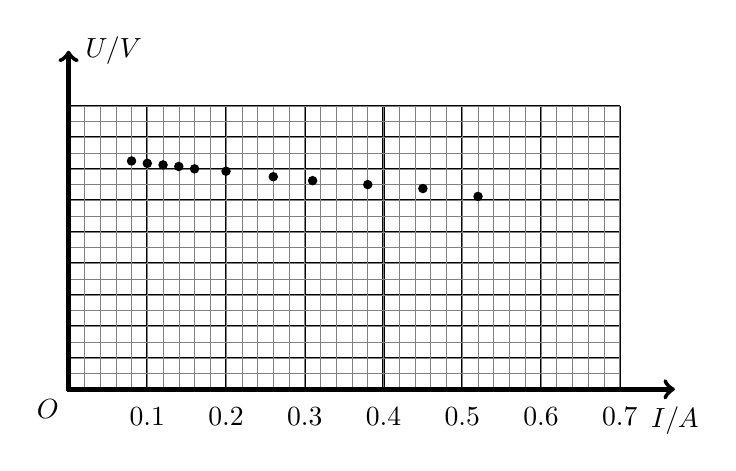
\begin{tikzpicture}
	\draw[thick,xstep=1cm,ystep=0.4cm] (0,0) grid (7,3.6); %主网格
	\draw[step=0.2cm,gray,very thin] (0,0) grid (7,3.6);%次网格
	
	\draw[ultra thick,->] (-0.02,0) -- (7.7,0) node [below =2pt] {$ I/A $} ; %横坐标轴
	\draw[ultra thick,->] (0,-0.02) -- (0,4.3)  node [right =2pt] {$ U/V $} ; %纵坐标轴
	\node at (0,0) [below left] {$ O $};%原点
	
	\foreach \xlabel in {1,2,...,7}{ %x轴刻度
		%\draw (\xlabel cm ,0.5pt) -- (\xlabel cm ,-0,5pt) ;
		\node[below=3pt]   at (\xlabel cm , 0) {$ 0.\xlabel $};
	}
	\foreach \ylabel in {0.4,0.8,1.2,1.6,2.0,2.4,2.8,3.2,3.6}{ %y轴刻度
		%\draw (-0.5pt,\ylabel cm) -- (0,5pt, \ylabel cm);
		\FPset\myy{\ylabel}%给计算的量赋值
		\FPeval{myresult}{trunc(myy/2:1)}%表达式计算,\FPprint\myresult显示
		\node[left=3pt]   at (0, \ylabel cm) {$ \FPprint\myresult  $};
	}
	
	\draw[fill] (0.8,2.9) circle [radius=1.5pt];
	\draw[fill] (1.0,2.87) circle [radius=1.5pt];
	\draw[fill] (1.2,2.85) circle [radius=1.5pt];
	\draw[fill] (1.4,2.83) circle [radius=1.5pt];
	\draw[fill] (1.6,2.80) circle [radius=1.5pt];
	\draw[fill] (2,2.77) circle [radius=1.5pt];
	\draw[fill] (2.6,2.7) circle [radius=1.5pt];
	\draw[fill] (3.1,2.65) circle [radius=1.5pt];
	\draw[fill] (3.8,2.6) circle [radius=1.5pt];
	\draw[fill] (4.5,2.55) circle [radius=1.5pt];
	\draw[fill] (5.2,2.45) circle [radius=1.5pt];
\end{tikzpicture}
\caption{}\label{2020:山东:14b}
\end{subfigure}
\end{figure}

\item 
针对电压表示数的变化范围比较小的问题,该小组利用实验室提供的器材改进了实验方案,重新
测量得到的数据如下表所示。

\begin{table}[h!]
\centering 
\begin{tabular}{|c|c|c|c|c|c|c|c|}
\hline 
序号 & 1 & 2 & 3 & 4 & 5 & 6 & 7
\\
\hline
$ I/A $ & 0.08 & 0.14 & 0.20 & 0.26 & 0.32 & 0.36 & 0.40
\\
\hline
$ U/V $& 1.35 & 1.20 & 1.05 & 0.88 & 0.73 & 0.71 & 0.52\\ 
\hline 
\end{tabular}
\end{table} 




请根据实验数据,回答以下问题:
\begin{enumerate}
%\renewcommand{\labelenumi}{\arabic{enumi}.}
% A(\Alph) a(\alph) I(\Roman) i(\roman) 1(\arabic)
%设定全局标号series=example	%引用全局变量resume=example
%[topsep=-0.3em,parsep=-0.3em,itemsep=-0.3em,partopsep=-0.3em]
%可使用leftmargin调整列表环境左边的空白长度 [leftmargin=0em]
\item
答题卡的坐标纸上已标出后 $ 3 $ 组数据对应的坐标点,请在答题卡的坐标纸上标出前 $ 4 $ 组数据对应的
坐标点并画出 $ U-I $ 图像。
\begin{figure}[h!]
	\centering
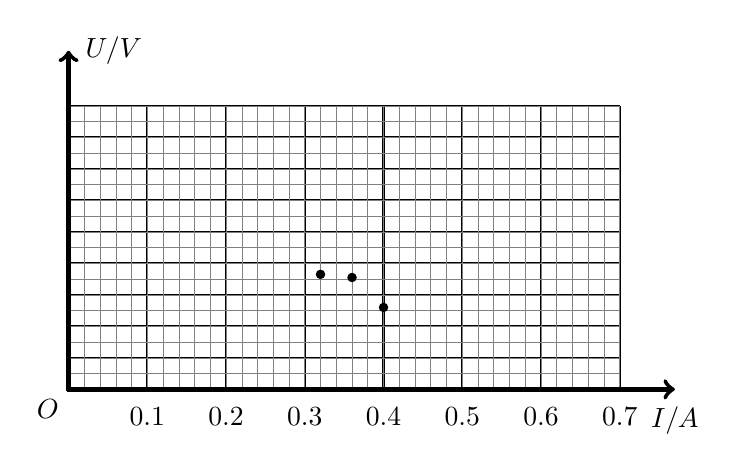
\begin{tikzpicture}
	\draw[thick,xstep=1cm,ystep=0.4cm] (0,0) grid (7,3.6); %主网格
	\draw[step=0.2cm,gray,very thin] (0,0) grid (7,3.6);%次网格
	
	\draw[ultra thick,->] (-0.02,0) -- (7.7,0) node [below =2pt] {$ I/A $} ; %横坐标轴
	\draw[ultra thick,->] (0,-0.02) -- (0,4.3)  node [right =2pt] {$ U/V $} ; %纵坐标轴
	\node at (0,0) [below left] {$ O $};%原点
	
	\foreach \xlabel in {1,2,...,7}{ %x轴刻度
		%\draw (\xlabel cm ,0.5pt) -- (\xlabel cm ,-0,5pt) ;
		\node[below=3pt]   at (\xlabel cm , 0) {$ 0.\xlabel $};
	}
	\foreach \ylabel in {0.4,0.8,1.2,1.6,2.0,2.4,2.8,3.2,3.6}{ %y轴刻度
		%\draw (-0.5pt,\ylabel cm) -- (0,5pt, \ylabel cm);
		 \FPset\myy{\ylabel}%给计算的量赋值
		 \FPeval{myresult}{trunc(myy/2:1)}%表达式计算,\FPprint\myresult显示
		\node[left=3pt]   at (0, \ylabel cm) {$ \FPprint\myresult  $};
	}
	
	\draw[fill] (4,1.04) circle [radius=1.5pt];
	\draw[fill] (3.6,1.42) circle [radius=1.5pt];
	\draw[fill] (3.2,1.46) circle [radius=1.5pt];
\end{tikzpicture}
\end{figure}


\item 
根据实验数据可知,所选的定值电阻为 \underlinegap (填“$ R_{1} $”或“$ R_{2} $”)。


\item 
用笔画线代替导线,请在答题卡上按照改进后的方案,将实物图连接成完整电路。
\begin{figure}[h!]
	\centering
	\includesvg[width=0.43\linewidth]{picture/svg/GZ-3-tiyou-1709}
\end{figure}

\end{enumerate}

	
\end{enumerate}


\tk{
\begin{enumerate}
%\renewcommand{\labelenumi}{\arabic{enumi}.}
% A(\Alph) a(\alph) I(\Roman) i(\roman) 1(\arabic)
%设定全局标号series=example	%引用全局变量resume=example
%[topsep=-0.3em,parsep=-0.3em,itemsep=-0.3em,partopsep=-0.3em]
%可使用leftmargin调整列表环境左边的空白长度 [leftmargin=0em]
\item
B	
\item 	
\begin{enumerate}
%\renewcommand{\labelenumi}{\arabic{enumi}.}
% A(\Alph) a(\alph) I(\Roman) i(\roman) 1(\arabic)
%设定全局标号series=example	%引用全局变量resume=example
%[topsep=-0.3em,parsep=-0.3em,itemsep=-0.3em,partopsep=-0.3em]
%可使用leftmargin调整列表环境左边的空白长度 [leftmargin=0em]
\item
如图:
\begin{center}
\includesvg[width=0.93\linewidth]{picture/svg/GZ-3-tiyou-0759} 
\end{center}
\item 
$ R_{1} $
\item 
如图:
\begin{center}
\includesvg[width=0.93\linewidth]{picture/svg/GZ-3-tiyou-1708} 
\end{center}
\end{enumerate}
\end{enumerate}
} 

%题目类型:实验
%题目难度:6
%题目区域:电路
%思想方法:
%题目特征:
%题目备注:



\newpage
\gaokaojs

\item
中医拔罐的物理原理是利用玻璃罐内外的气压差使罐吸附在人体穴位上,进而治疗某些疾病。
常见拔罐有两种,如图所示,左侧为火罐,下端开口;右侧为抽气拔罐,下端开口,上端留有抽气阀
门。使用火罐时,先加热罐中气体,然后迅速按到皮肤上,自然降温后火罐内部气压低于外部大气压,
使火罐紧紧吸附在皮肤上。抽气拔罐是先把罐体按在皮肤上,再通过抽气降低罐内气体压强。某次使
用火罐时,罐内气体初始压强与外部大气压相同,温度为 $ 450 \ K $,最终降到 $ 300 \ K $,因皮肤凸起,内
部气体体积变为罐容积的$ \frac{20}{21} $。若换用抽气拔罐,抽气后罐内剩余气体体积变为抽气拔罐容积的$ \frac{20}{21} $,
罐内气压与火罐降温后的内部气压相同。罐内气体均可视为理想气体,忽略抽气过程中气体温度的变
化。求应抽出气体的质量与抽气前罐内气体质量的比值。
\begin{figure}[h!]
\flushright
\includesvg[width=0.35\linewidth]{picture/svg/GZ-3-tiyou-0752}
\end{figure}


\banswer{
$\frac{\Delta m}{m}=\frac{1}{3}$
}

%题目类型:计算
%题目难度:6.5
%题目区域:热学:理想气体状态方程
%思想方法:
%题目特征:材料分析
%题目备注:


\newpage
\item 
单板滑雪 $ U $ 型池比赛是冬奥会比赛项目,其场地可以简化为如图 \subref{2020:山东:16a} 所示的模型$ :U $ 形滑道由两
个半径相同的四分之一圆柱面轨道和一个中央的平面直轨道连接而成,轨道倾角为 $ 17.2 ^{ \circ } $。某次练习
过程中,运动员以 $ v_{M}=10 \ m/s $ 的速度从轨道边缘上的 $ M $ 点沿轨道的竖直切面 $ ABCD $ 滑出轨道,速度方
向与轨道边缘线 $ AD $ 的夹角$ \alpha =72.8 ^{ \circ } $,腾空后沿轨道边缘的 $ N $ 点进入轨道。图 \subref{2020:山东:16b} 为腾空过程左视图。
该运动员可视为质点,不计空气阻力,取重力加速度的大小 $ g=10 \ m/s^{2}, \sin 72.8 ^{ \circ } =0.96 $,$ \cos 72.8 ^{ \circ } =0.30$。求:
\begin{enumerate}
%\renewcommand{\labelenumi}{\arabic{enumi}.}
% A(\Alph) a(\alph) I(\Roman) i(\roman) 1(\arabic)
%设定全局标号series=example	%引用全局变量resume=example
%[topsep=-0.3em,parsep=-0.3em,itemsep=-0.3em,partopsep=-0.3em]
%可使用leftmargin调整列表环境左边的空白长度 [leftmargin=0em]
\item
运动员腾空过程中离开 $ AD $ 的距离的最大值 $ d $;
\item 
$ M $、$ N $ 之间的距离 $ L $。
\end{enumerate}
\begin{figure}[h!]
\flushright
\begin{subfigure}{0.4\linewidth}
\centering
\includesvg[width=0.85\linewidth]{picture/svg/GZ-3-tiyou-0754} 
\caption{}\label{2020:山东:16a}
\end{subfigure}
\begin{subfigure}{0.4\linewidth}
\centering
\includesvg[width=0.95\linewidth]{picture/svg/GZ-3-tiyou-0755} 
\caption{}\label{2020:山东:16b}
\end{subfigure}
\end{figure}



\banswer{
\begin{enumerate}
%\renewcommand{\labelenumi}{\arabic{enumi}.}
% A(\Alph) a(\alph) I(\Roman) i(\roman) 1(\arabic)
%设定全局标号series=example	%引用全局变量resume=example
%[topsep=-0.3em,parsep=-0.3em,itemsep=-0.3em,partopsep=-0.3em]
%可使用leftmargin调整列表环境左边的空白长度 [leftmargin=0em]
\item
$d=4.8 \ m$	
\item 
$L=12 \ m$
\end{enumerate}
}


%题目类型:计算
%题目难度:7
%题目区域:曲线运动:斜抛
%思想方法:
%题目特征:材料分析
%题目备注:




\newpage
\item
某型号质谱仪的工作原理如图 \subref{2020:山东:17a} 所示。$ M $、$ N $ 为竖直放置的两金属板,两板间电压为 $ U,Q $ 板
为记录板,分界面 $ P $ 将 $ N $、$ Q $ 间区域分为宽度均为 $ d $ 的 \lmd{1} 、 \lmd{1} 两部分,$ M $、$ N $、$ P $、$ Q $ 所在平面相互平行,
$ a $、$ b $ 为 $ M $、$ N $ 上两正对的小孔。以 $ a $、$ b $ 所在直线为 $ z $ 轴, 向右为正方向,取 $ z $ 轴与 $ Q $ 板的交点 $ O $ 为坐
标原点,以平行于 $ Q $ 板水平向里为 $ x $ 轴正方向,竖直向上为 $ y $ 轴正方向,建立空间直角坐标系 $ Oxyz $。
区域 \lmd{1} 、$ \lmd{2} $内分别充满沿 $ x $ 轴正方向的匀强磁场和匀强电场,磁感应强度大小、电场强度大小分别为 $ B $和 $ E $。一质量为 $ m $,电荷量为$ +q $ 的粒子,从 $ a $ 孔飘入电场(初速度视为零),经 $ b $ 孔进入磁场,过 $ P $ 面
上的 $ c $ 点(图中未画出)进入电场,最终打到记录板 $ Q $ 上。不计粒子重力。
\begin{enumerate}
%\renewcommand{\labelenumi}{\arabic{enumi}.}
% A(\Alph) a(\alph) I(\Roman) i(\roman) 1(\arabic)
%设定全局标号series=example	%引用全局变量resume=example
%[topsep=-0.3em,parsep=-0.3em,itemsep=-0.3em,partopsep=-0.3em]
%可使用leftmargin调整列表环境左边的空白长度 [leftmargin=0em]
\item
求粒子在磁场中做圆周运动的半径 $ R $ 以及 $ c $ 点到 $ z $ 轴的距离 $ L $;
\item 
求粒子打到记录板上位置的 $ x $ 坐标;
\item 
求粒子打到记录板上位置的 $ y $ 坐标(用 $ R $、$ d $ 表示);
\item 
如图 \subref{2020:山东:17b} 所示,在记录板上得到三个点 $ s_{1} $、$ s_{2} $、$ s_{3} $,若这三个点是质子 \ce{^{1}_{1}H} 、氚核 \ce{^{3}_{1}H} 、氦核 \ce{^{4}_{2}He} 的位
置,请写出这三个点分别对应哪个粒子(不考虑粒子间的相互作用,不要求写出推导过程)。

\end{enumerate}
\begin{figure}[h!]
\flushright
\begin{subfigure}{0.4\linewidth}
\centering
\includesvg[width=0.8\linewidth]{picture/svg/GZ-3-tiyou-0756} 
\caption{}\label{2020:山东:17a}
\end{subfigure}
\begin{subfigure}{0.4\linewidth}
\centering
\includesvg[width=0.6\linewidth]{picture/svg/GZ-3-tiyou-0757} 
\caption{}\label{2020:山东:17b}
\end{subfigure}	
\end{figure}


\banswer{
\begin{enumerate}
%\renewcommand{\labelenumi}{\arabic{enumi}.}
% A(\Alph) a(\alph) I(\Roman) i(\roman) 1(\arabic)
%设定全局标号series=example	%引用全局变量resume=example
%[topsep=-0.3em,parsep=-0.3em,itemsep=-0.3em,partopsep=-0.3em]
%可使用leftmargin调整列表环境左边的空白长度 [leftmargin=0em]
\item
$R=\frac{\sqrt{2 m q U}}{q B}$ \quad $L=\frac{\sqrt{2 m q U}}{q B}-\sqrt{\frac{2 m U}{q B^{2}}-d^{2}}$
\item 
$x=\frac{m d^{2} E}{4 m U-2 q d^{2} B^{2}}$
\item 
$y=R-\sqrt{R^{2}-d^{2}}+\frac{d^{2}}{\sqrt{R^{2}-d^{2}}}$
\item 
$s_{1} $、$ s_{2}$、$ s_{3}$ 分别对应气核 ${ }_{1}^{3} \mathrm{H}$、氦去 ${ }_{2}^{4} \mathrm{He}$、质子 ${ }^{1}_{1} \mathrm{H}$ 的位置
\end{enumerate}
}

%题目类型:计算
%题目难度:6.5
%题目区域:磁场:磁场中带电粒子的运动
%思想方法:
%题目特征:材料分析:计算练习
%题目备注:用运动的分解




\newpage
\item
如图所示,一倾角为$ \theta $的固定斜面的底端安装一弹性挡板,$ P $、$ Q $ 两物块的质量分别为 $ m $ 和
$ 4m $,$ Q $ 静止于斜面上 $ A $ 处。某时刻,$ P $ 以沿斜面向上的速度 $ v_{0} $ 与 $ Q $ 发生弹性碰撞。$ Q $ 与斜面间的动摩
擦因数等于 $ \tan \theta $,设最大静摩擦力等于滑动摩擦力。$ P $ 与斜面间无摩擦,与挡板之间的碰撞无动能损
失。两物块均可以看作质点,斜面足够长,$ Q $ 的速度减为零之前 $ P $ 不会与之发生碰撞。重力加速度大
小为 $ g $。
\begin{enumerate}
%\renewcommand{\labelenumi}{\arabic{enumi}.}
% A(\Alph) a(\alph) I(\Roman) i(\roman) 1(\arabic)
%设定全局标号series=example	%引用全局变量resume=example
%[topsep=-0.3em,parsep=-0.3em,itemsep=-0.3em,partopsep=-0.3em]
%可使用leftmargin调整列表环境左边的空白长度 [leftmargin=0em]
\item
求 $ P $ 与 $ Q $ 第一次碰撞后瞬间各自的速度大小 $ v _{P1} $、$ v _{Q1} $;
\item 
求第 $ n $ 次碰撞使物块 $ Q $ 上升的高度 $ h_n $;
\item 
求物块 $ Q $ 从 $ A $ 点上升的总高度 $ H $;
\item 
为保证在 $ Q $ 的速度减为零之前 $ P $ 不会与之发生碰撞,求 $ A $ 点与挡板之间的最小距离 $ s $。
\end{enumerate}
\begin{figure}[h!]
\flushright
\includesvg[width=0.4\linewidth]{picture/svg/GZ-3-tiyou-0758}
\end{figure}

\banswer{
\begin{enumerate}
%\renewcommand{\labelenumi}{\arabic{enumi}.}
% A(\Alph) a(\alph) I(\Roman) i(\roman) 1(\arabic)
%设定全局标号series=example	%引用全局变量resume=example
%[topsep=-0.3em,parsep=-0.3em,itemsep=-0.3em,partopsep=-0.3em]
%可使用leftmargin调整列表环境左边的空白长度 [leftmargin=0em]
\item
$v_{P 1}=-\frac{3}{5} v_{0}$ \quad 
$v_{Q 1}=\frac{2}{5} v_{0}$
\item 
$h_{1}=\frac{v_{0}^{2}}{25 g}$ \\
 $h_{2}=\frac{7}{25} \cdot \frac{v_{0}^{2}}{25 g}$ \\
 $h_{3}=\left(\frac{7}{25}\right)^{2} \cdot \frac{v_{0}^{2}}{25 g}$\\
总结可知,第 $n$ 次碰撞后,物块 $Q$ 上升的高度为:\\
$h_{n}=\left(\frac{7}{25}\right)^{n-1} \cdot \frac{v_{0}^{2}}{25 g} \quad(n=1,2,3 \cdots \cdots)$
\item 
$s=\frac{(8 \sqrt{7}-13) v_{0}^{2}}{200 g \sin \theta}$
\end{enumerate}	
}

%题目类型:计算
%题目难度:3
%题目区域:能量守恒:动量
%思想方法:极限
%题目特征:计算练习
%题目备注:




\end{enumerate}

